\section{Introduction}
\label{sec:intro}
%it has been suggested that animals possess languages in their communications with others\MY{this is a bold argument, rephrase: animals use vocal expressions to communicate, also refs needed here}. 
Animal languages have captured the curiosity of scientists for years and animals use vocal expressions to communicate ~\cite{garcia2017animal}.
Despite various attempts from diverse perspectives, deciphering the intricately complex semantic meanings within animal communication systems remains a challenge ~\cite{andreas2022towards,scott2023animal}. Acquiring a deeper comprehension of animal language holds significant implications for unraveling their social structures, and intelligence, and facilitating human-animal interactions. 

Within the expansive realm of animal languages, the study of \textbf{dog language} holds particular interest. Dogs, as one of the most popular and widely kept pets, engage in constant interaction with human beings through their vocal expressions.
Given the massive interactions between dogs and people during the domestication process, dogs' vocal behavior undergoes considerable changes ~\cite{jieyiacl2023, feddersen2000vocalization} and it is reasonable to infer that diverse sounds emitted by dogs in varying scenes carry distinct significances. Previous works on dog language have largely relied upon experimental knowledge and heuristic
subjective observations, which depend on long-term experiences and costly data-collection and can be limited and prone to biases ~\cite{yin2002new,pongracz2010barking,farago2017dog}. Only coarse-grained meanings can be drawn given limited data and corresponding scenes from these studies. Our web-data-driven exploration leverages a more comprehensive methodology to uncover finer-grained semantics with a broader context. The utilization of \textbf{web data} offers a wealth of information, introducing numerous possible variables and semantic clues, thus enabling a more comprehensive analysis. 

%\MY{Only coarse-grained meanings can be drawn given limited data and corresponding scenes from these studies.}
\begin{figure*}[t]
	\centering
	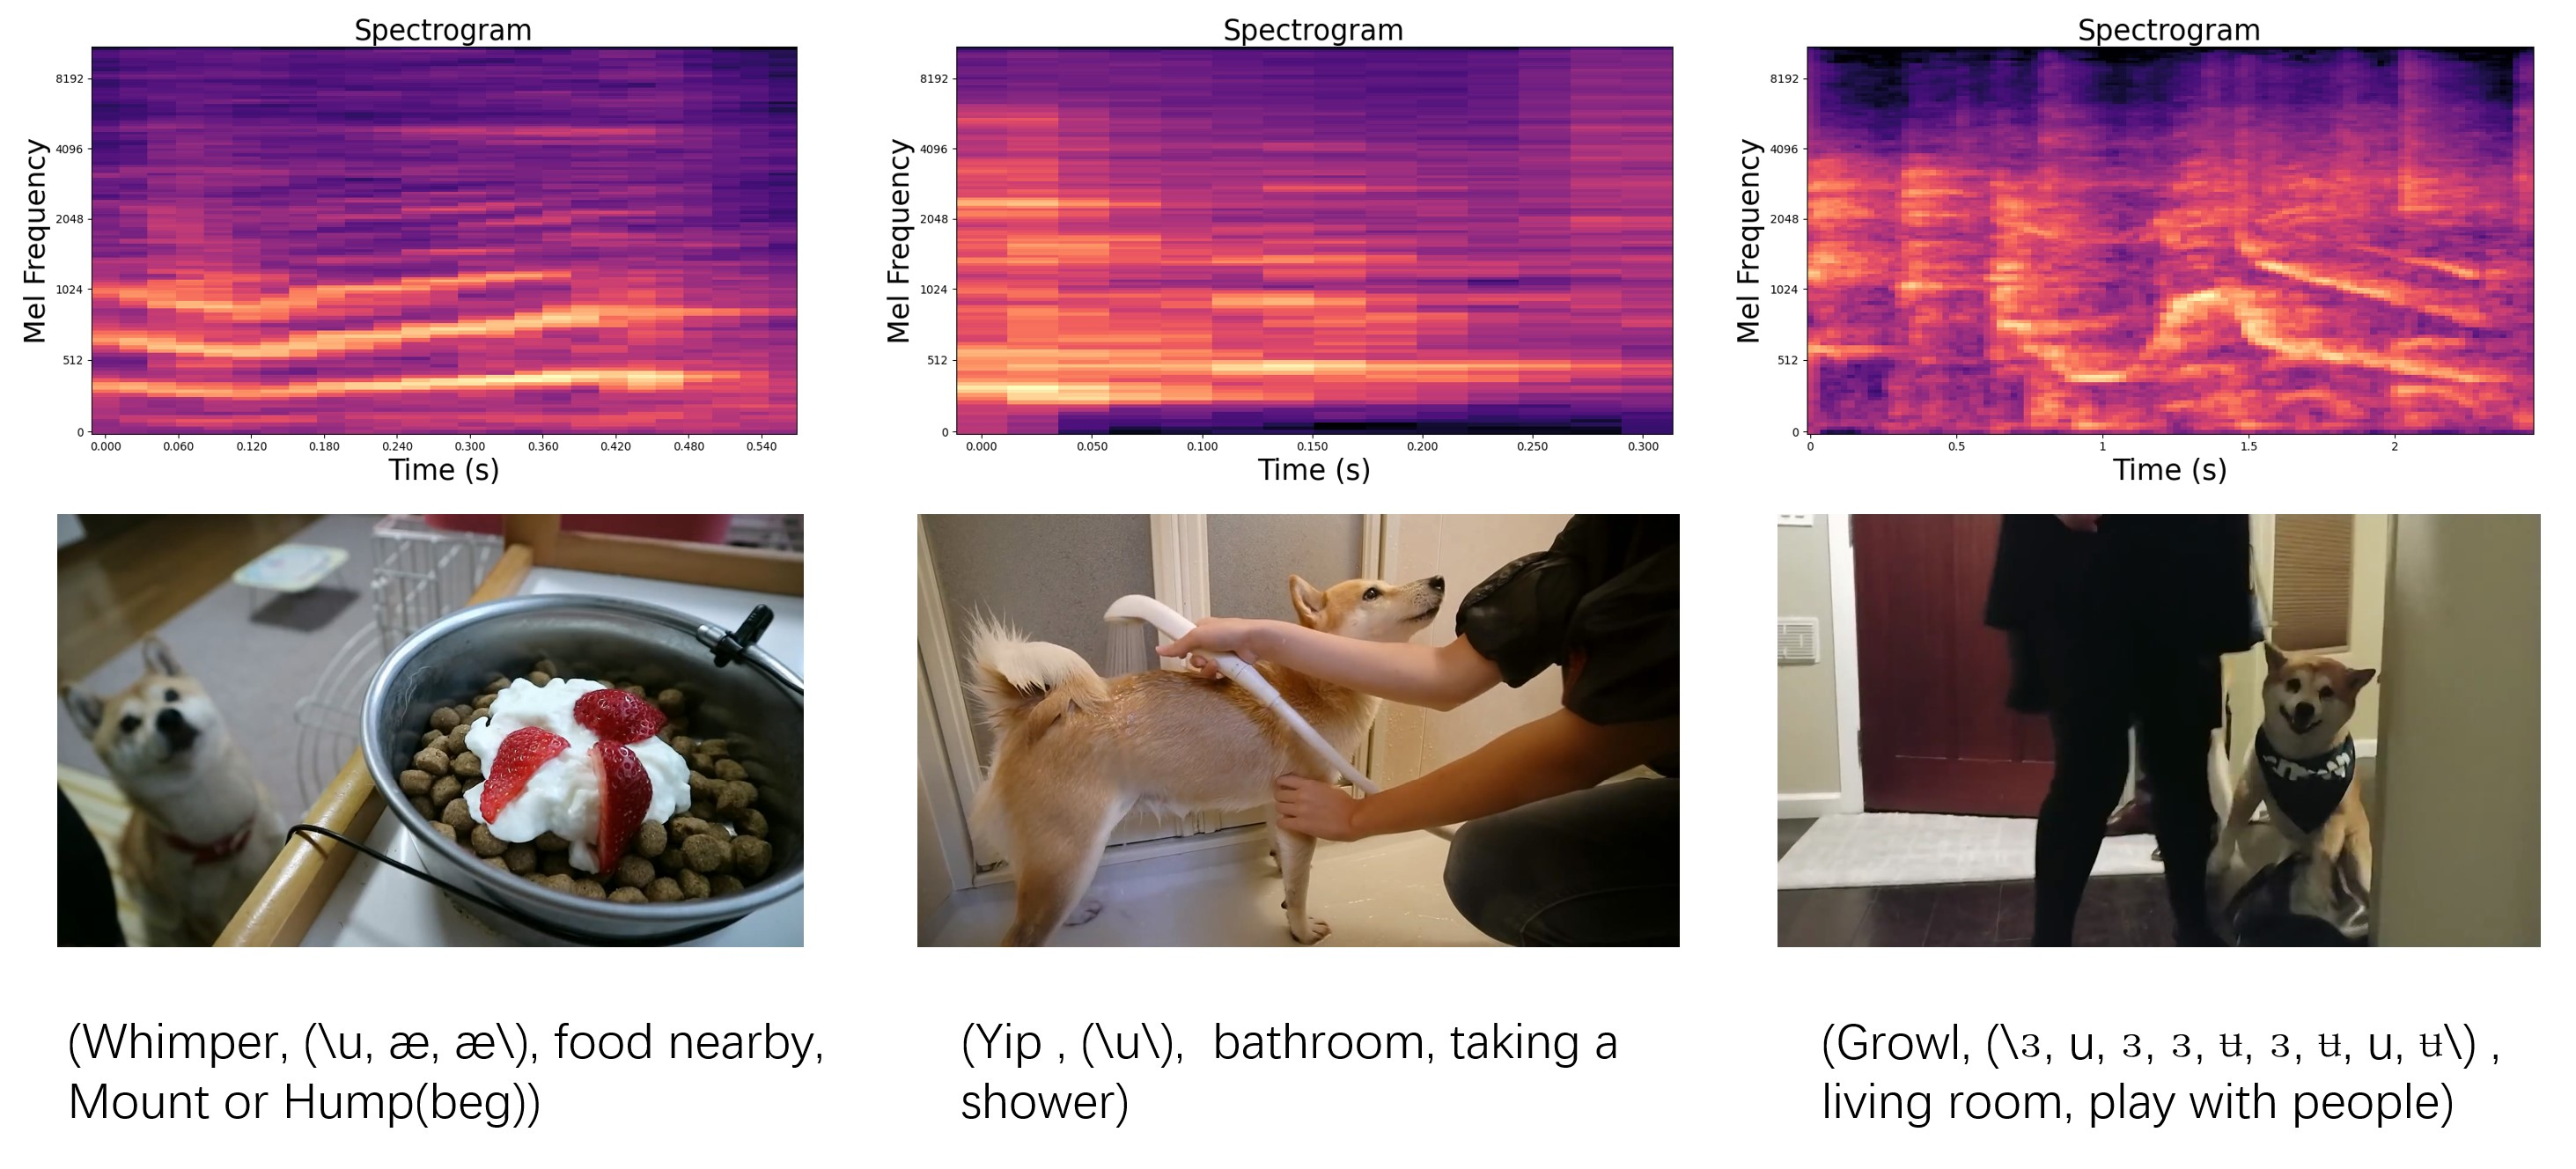
\includegraphics[width=0.85\textwidth]{images/intro.jpg}
	\caption{Introducing scenario: Spectrograms of dog sounds in the corresponding context. When the dog is begging for food, taking a shower, or playing with people, its vocal spectrograms differ a lot. We map possible words and subwords extracted from dog barking audio with location and activity, forming our quadruplet dataset.  %\MY{please use \textbackslash u\textbackslash  wherever you mention phoneme symbols}
\texttt{<word, IPA symbols, location, activity>}.
%		\href{https://anonymous.4open.science/r/emnlp2023-937942/audios_in_paper/fig11.wav}{[Listen 1]}
%		\href{https://anonymous.4open.science/r/emnlp2023-937942/audios_in_paper/fig12.wav}{[Listen 2]}
%		\href{https://anonymous.4open.science/r/emnlp2023-937942/audios_in_paper/fig13.wav}{[Listen 3]}
	} %\MY{you need subfigure titles, e.g. ``Bow-wow''  under spectrogram, ``Food nearby, laying down'' under 1st picture}}
	%\KZ{Pls leave some spaces between the 3 pics on the bottom.}
	%to anywhere in the text! Every fig and table that you include in the paper must
	%be referred to somewhere!}}
	\label{fig:intropic}
\end{figure*}

There is a wide range of vocalizations dogs can produce ~\cite{yeon2007vocal}, which are affected by various engaged objects, the emotion of the dog, the surrounding environment the dog is located in, the activity the dog is doing, the object the dog interacts with, and even the age and gender of the dog may play a key factor ~\cite{pongracz2005human,molnar2009dogs}. 
Given the benefits of using web data, we opt to focus on the Shiba Inu breed for our research as Shiba Inu is a widely adopted dog at home and plenty of video data is available on YouTube. Hereby, we investigate the semantic meaning of the Shiba Inu dog sound according to two important factors of the context, the \textbf{location} and the \textbf{activity} of the dog as these two factors are currently available. 
%\MY{this is not a complete sentence, There are a wide range of ...can produce, which are affected/influenced by xxxx.}
%\MY{how is this different from``engating with the external environment'', not quite clear from current text}
%\MY{not only available..but we need to say these are the two most prominent factors influencing possible semantics, add this in and see if you can find any refs supporting this argument}. 
%\AT{can not find refs, only find situation may influnce}
%whereas other factors are difficult to extract from online videos. 
%\MY{we didn't talk about why social media data is helpful, u can talk about this in previous paragraph or maybe before saying shiba inu. say that web data provides a lot of information about the possible variables or semantic clues}
%\MY{why we limit to these two factors? due to ambiguity in other factors...}

 %\KZ{Give cites here.} 
 
%\JY{here add our advantages over previous work}

To understand the semantic meaning of dog language, previous works always record dog sounds in different scenarios and then analyze them. As we have online videos, there are several challenges: extract the meaningful dog sound and context from videos and ascertain if they show consistent patterns with context. In this work, we implement the first data-driven, evidence-based research sourced from social media to give fine-grained semantics to understand the vocal language of Shiba Inu. We construct data as ~\figref{fig:intropic} for our dataset to map dog sound with context which enables us to take a closer look into the behaviors of animals and some hidden \textbf{semantic patterns}. For example, one kind of dog sound, bow-wow, is usually mixed with bark by previous researchers. However, in our work, we find that it shows the curiosity of dogs for the surroundings while bark does not exhibit such meaning. 
% In comparison, we propose a web-data-driven method that takes advantage of the large Internet resources, which saves collection costs as well as enlarges our data size. 
%\MY{add a sentence explaining this figure, and we have to say somewhere that current dataset consists of six different sound types}. With data collected from the internet
%\MY{haven't talked about data quantity by far} 
%Another example is related to ``growl'', traditionally seen as a low, guttural vocalization produced by animals as a warning, a sign of aggression, or to express anger\footnote{https://en.wikipedia.org/wiki/Growling}, while our analysis shows that ``growl'' for dogs may also be seen as a signal of positively interacting with humans. 
On the other hand, our method has more detailed contexts for analyzing animal languages, which will benefit future works. We identified as many as 11 locations and 14 activities, in which dogs might produce 6 different vocal sounds to signify various meanings. To associate vocal expression patterns with possible lexical meanings, we need to respectively extract vocal sounds and their transcriptions as well as the activity and location that might give rise to a change of meanings. With these fine-grained labels, we can capture subtle semantic differences and constant vocal patterns under these contexts to explore the semantics of vocalizations for Shiba Inu dogs.
Our main contributions can be summarized as follows:
 %\MY{make some text bold in intro and contribution, where important and needs reviewers' special attention}
%\MY{with these fine-grained labels, we can capture subtle semantic differences and constant vocal patterns under these contexts}
%\KZ{You were already talking about gowling in the first para,now setting the stage for dog language seems too late.}
 
%\KZ{A bit too verbose here for giving the reason why we study dog language.
%I think the first two paras can be shortened and combined into one.}
%\MY{ In the 1st paragraph, you should focus on saying that why problem is important and why it is difficult to solve given previous effors. }
%\KZ{You need to cite more papers in the intro. At least cite two of Jieyi's
%papers?}


%\KZ{Why previous approach doesn't work well. E.g., bark and bow-wow are
%complicated and have not been given clear semantics.} explain above!!!

%Dog sounds can be classified into different types. The classification of these sounds is a interesting task, as it provides a framework for understanding the diverse vocal manifestations of dogs. We adopt the classification defined in Audioset, where dog sounds can be categorized into bark, yip, howl, bow-wow, growling, and whimper. Each of these categories present distinct vocal patterns of dogs, each carrying unique semantic connotations. Dogs will make different sound in different context. Here, we consider context to be determined by the actions of the dog at that time and the scene in which it is located. 
%\MY{You are correct that we need to say that verbal communications are to interact with outside world, hence we define the context i.e. their locations, and activity to analyse these interactions with certain words. Better give a few references that preliminary investigations indicate that dogs' sound are different given these conditions. }

 %\MY{This and the later para can be merged together, you don't want to go deep into too many details here to distract your readers}
%i.e., using same words under same context, we would determine that 
%these words are used to express certain meanings.  
%\KZ{The following two paras can be more concise.}



%\MY{This para is still verbose and detailed, you summarize your main idea in tackling the problem, and illustrate it here.}

 %to infer the context of the words we have extracted and to match the words and the context, 
%To tackle the challenges in aligning words with context, we process the audio to find words and remove the noisy parts then we classify these words into different types. Then, according to the corresponding words' timestamp, we go back to videos to find the activity and location (as shown in ~\figref{fig:intropic}).
%The classification of the words provides us with a framework for understanding the diverse vocal manifestations of dogs. 
%We adopt the definition of Audioset ~\cite{gemmeke2017audio}, where dog words can be categorized into the bark, yip, howl, bow-wow, growling, and whimper. 
%We analyze them in accordance with the corresponding context where a specific sound is produced. 

%For example, howl is used when there is food nearby, so it may implicate the desire for food. 
%We also explore sequences of words to find bi-gram semantic meaning. Some of our results support previous findings. For example, ``whimper'' can express attention seeking. We also yield new possible discoveries. For example, ``howl'' can be used as a signal for food. We aim to deepen our understanding of the complex communication system employed by dogs and eventually decipher their language by exploring the possible dog word meaning.
%\MY{Some of our results support previous findings that xxxx. We also yield new possible discoveries that xxx}

%Each of these categories present distinct vocal patterns and possible different meanings. Bark is the principal communication sound produced by dogs; Yip is a sharp high-pitched bark or cry, typically from a miniature dog; Howl is the long plaintive cry of a dog; Bow-wow is more tonal and less abrupt than a classic bark; Growling is a low, guttural vocalization; and whimper is a muted dog vocaliazation indicating submission, fear or pain.




%\JY{add their definitions and meanings here}
%For example, when the dog is running for fight, it will bark loudly with high frequency. Whereas begging for food, it will whimper with a soft and low voice. 

%\begin{table}[th]
%	\small
%	\begin{tabular}{p{0.15\columnwidth}|p{0.35\columnwidth}|p{0.35\columnwidth}}
%		\toprule
%		\textbf{Word} & \textbf{Definition} & \textbf{Meaning}\\ \midrule
%		Bark & ?
%		\\ \midrule
%		Yip & 
%		\\ \midrule
%		Howl &
%		\\\midrule
%		Bow-wow & 
%		\\\midrule
%		Growling & 
%		\\\midrule
%		Whimper & 
%		\\
%		\bottomrule
%	\end{tabular}
%	\caption{Overall findings of the analysis.}
%	\label{tab:worddefinition}
%\end{table}


%\MY{See? this para is somewhat lost, as previously it seems you have talked about how you aligned them and drew the conclusions, and now you start again talking about the triplets}
%\MY{This detailed explaination to our work can come later in the intro. Here you would say that the challenging part in understanding animal vocalization is to segment and extract meaningful words. By matching these distinct types of words to context, we can provide initial discoveries to animal semantics, that if they show consistent patterns, i.e. using same words under same context, we would determine that these words are used to express certain meanings}

\begin{itemize}
	\item We propose a universal pipeline to process and analyze dog-related videos on YouTube to understand the lexical semantics of dog language. The framework is reusable to other animal species for which videos are available.
\item We are the first to implement data-driven research to study dog semantic language from web data. We build a dataset of 10,779 quadruplets that contains 6 distinct words, subwords, and corresponding context for exploring dog language. We define fine-grained 14 activities and 11 locations that could imply different semantic meanings which can be extracted from videos. 
\item Through our investigation of dog sound patterns, we have uncovered several conclusions that align with existing human knowledge and previous research. Additionally, we have gained some unique insights that have been under-explored. 
%\MY{add exact numbers here to show largest, and section numbers in the main text}
%\MY{we could say that we define fine-grained activities and locations that could imply different semantic meanings, and these are computable (can be extracted from videos)}
%We furthur find the minimal semantic unit for Shiba Inu dogs. 
%\KZ{Very strong claim: We furthur find the minimal semantic units for the dog language.} 
%\footnote{Code and dataset can be seen at \url{https://anonymous.4open.science/r/emnlp2023-937942/README.md}} 
\end{itemize}

%\cite{Gusfield:97}
